\chapter{Implementation} \label{implementation}

For this project I implemented the design as described in the previous chapter.
It is a command line application that takes a source code file as input and
performs semantic analysis on its \gls{ast}. I chose to write my implementation
using the Rust programming language. It is a memory safe language that leverages
the LLVM backend for highly optimized code. This makes it easy to write
robust and performant code. It additionally has very good parallel programming
facilities and an extensive software ecosystem that makes it ideal for this kind
of project. 

Section \ref{structure}
\newline \newline
Section \ref{dependancies}
\newline \newline
Section \ref{outputs_and_visualizations}
\newline \newline
Section \ref{debugging}

\section{Dependencies} \label{dependancies}

Code dependencies in the Rust code ecosystem that are  available through the
cargo package manager are called crates. These crates are comparable to small,
open source, third party libraries that can easily be integrated into a rust
project. In this section I mention the code dependencies I've used in my
implementation in order to illustrate what parts of my project were accomplished
through the use of third party code.

\subsection{Core}

\textbf{crossbeam} - Common data structures for implementing parallel systems.
This crate implements a concurrently accessible queue, skiplist and a
multi-producer, multi-consumer message passing channel. All of these data
structures are important for reliably sharing data across threads.
\newline\newline
\textbf{regex-syntax} - A crate for parsing standard regular expression syntax.
It provides a simple \gls{ast} that the lexer uses to read the mappings from
lexemes to regular expression patterns.
\newline\newline
\textbf{dot} - A crate that makes it easier to generate graphs in the dot
language. Its used to visualise the parse tree and \gls{ast}.
\gls{ast}.
\newline\newline
\textbf{criterion} - Reliable benchmarking facilities for testing the performance of the
compiler with differently sized inputs.

\subsection{Utility or Minor Contribution}
\textbf{tinyrand} - A lightweight implementation of random number
generation. It is used for creating unique IDs for bathes of work in the work
queue.
\textbf{serde} - Serialization and deserialization capabilities for transferring
code to and from the javascript runtime when running in the browser.
\newline\newline
\textbf{wasm-bindgen} - Macro's for easily creating bindings to javascript when
compiling to web assembly.
\newline\newline
\textbf{log, flexi\_logger ,wasm\-logger, console\_error\_panic\_hook} - Various
crates for logging to files as well as to the terminal, improved formatting and
correct logging when running in the browser.
\newline\newline
\textbf{simple-error} - A simple library for creating errors from error messages
instead of creating types for every error.

\subsection{Optimisation}
\textbf{memmap} - An interface for using linux's memmap syscall. Using memap to
read large files is  faster than using the standard read syscall.
\newline\newline
\textbf{bittyset} - A set implementation that uses a bit vector as a backing
store. This enables a compact representation as well as faster set operations in
the parser where sets of terminals and non-terminals are used.

\section{Structure} \label{structure}
\subsection{Lexical Analyser}
\subsubsection{NFA Generation}
\subsubsection{DFA Generation}
\subsection{Parser}
\subsubsection{Generating the Operator Precedence Table}
\subsubsection{Parsing Grammar Transformation} \label{parsing_grammar_transformation}
\subsection{Semantic Semantic Analysis}

\section{Outputs and Visualizations} \label{outputs_and_visualizations}

\section{Debugging} \label{debugging}

The Rust code in the fern repository showcases a comprehensive implementation of
a language processing system, including lexical analysis, parsing, and possibly
semantic analysis and code generation. Here's an overview of the implementation
based on the provided Rust code files: Key Components:
Lexical Analysis (src/lexer.rs, src/grammar/lg.rs)

    Lexer Implementation: The lexer component is responsible for tokenizing
the input source code. It uses a set of rules defined in src/grammar/lg.rs to
match patterns in the input text and convert them into tokens. This process is
crucial for the parsing stage, as it simplifies the input by abstracting away
the textual representation into a series of tokens with assigned meanings.

Parsing (src/parser.rs, src/parsetree.rs)
    Parser and Parse Tree: The parser takes the tokens generated by the lexer
    and constructs a parse tree based on the grammar of the language being
    analyzed. This tree represents the syntactic structure of the input code.
    The implementation in src/parser.rs and src/parsetree.rs likely involves
    recursive descent parsing or another parsing technique to handle the
    language's grammar.

Semantic Analysis (src/analysis.rs)

    Analysis: After parsing, the src/analysis.rs file suggests that the code
performs some form of semantic analysis. This could involve checking variable
declarations before use, type checking, or other compile-time checks that ensure
the program's semantic correctness.

Intermediate Representation (src/ir.rs)

    Intermediate Representation (IR): The src/ir.rs file indicates the
generation of an intermediate representation of the code. IR is a lower-level
representation of the program that is easier for a compiler or interpreter to
optimize and translate into machine code or another target language.

Language Specific Implementations (src/eslang.rs, src/json.rs, src/fern.rs)

    Language Implementations: The repository includes specific implementations
for different languages or formats, such as a custom language (src/eslang.rs),
JSON (src/json.rs), and possibly "fern" itself (src/fern.rs). These files
contain the rules and logic for parsing and analyzing these specific languages.

Implementation Overview for Report:
In your report's implementation section, you could describe how the project
is structured around the core components of a compiler or interpreter: lexical
analysis, parsing, semantic analysis, and intermediate representation. Highlight
the modular design that allows for the processing of different languages, as
evidenced by the separate implementations for each language. Discuss the use of
Rust's powerful type system and ownership model to manage resources efficiently
and ensure memory safety throughout the compilation process.

You might also want to mention the use of external libraries (if any are used)
and how they integrate with the project's codebase to enhance functionality,
such as for parallel processing or handling complex data structures.

Finally, consider discussing the project's testing strategy, based on the
presence of tests/ and benches/ directories, to ensure the reliability and
performance of the language processing system.

Would you like more detailed information or assistance with another part of
your report?

\begin{listing}[H]
\begin{minted}[linenos]{text}
fn factorial[n: int] {
    if n == 0 {
        return 1;
    % } 

    return (n * factorial(n - 1));
}
\end{minted}
\caption{Factorial in the test language.}
\label{lst:factorial_example}
\end{listing}

\begin{listing}[H]
\begin{minted}[linenos]{json}
{
  "a": 100,
  "b": {
    "x": [
      100,
      "a"
    ]
  }
}
\end{minted}
\caption{Example of parsable JSON.}
\hrulefill
\label{lst:json_example}
\end{listing}

\begin{figure}[t]
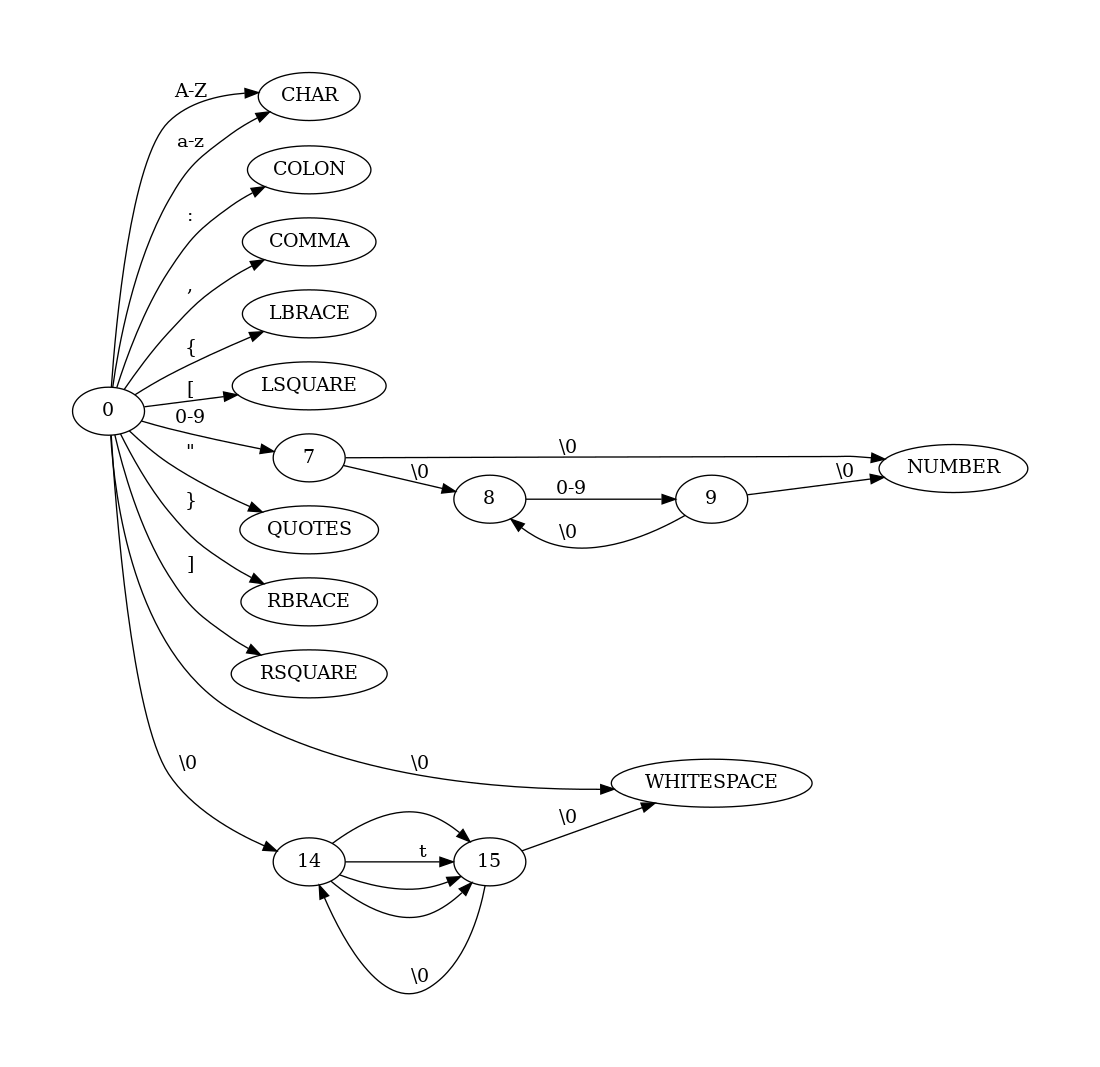
\includegraphics[width=\linewidth]{images/nfa.png}
\caption{NFA of the lexical grammar}
\label{fig:nfa}
\end{figure}

\begin{figure}[t]
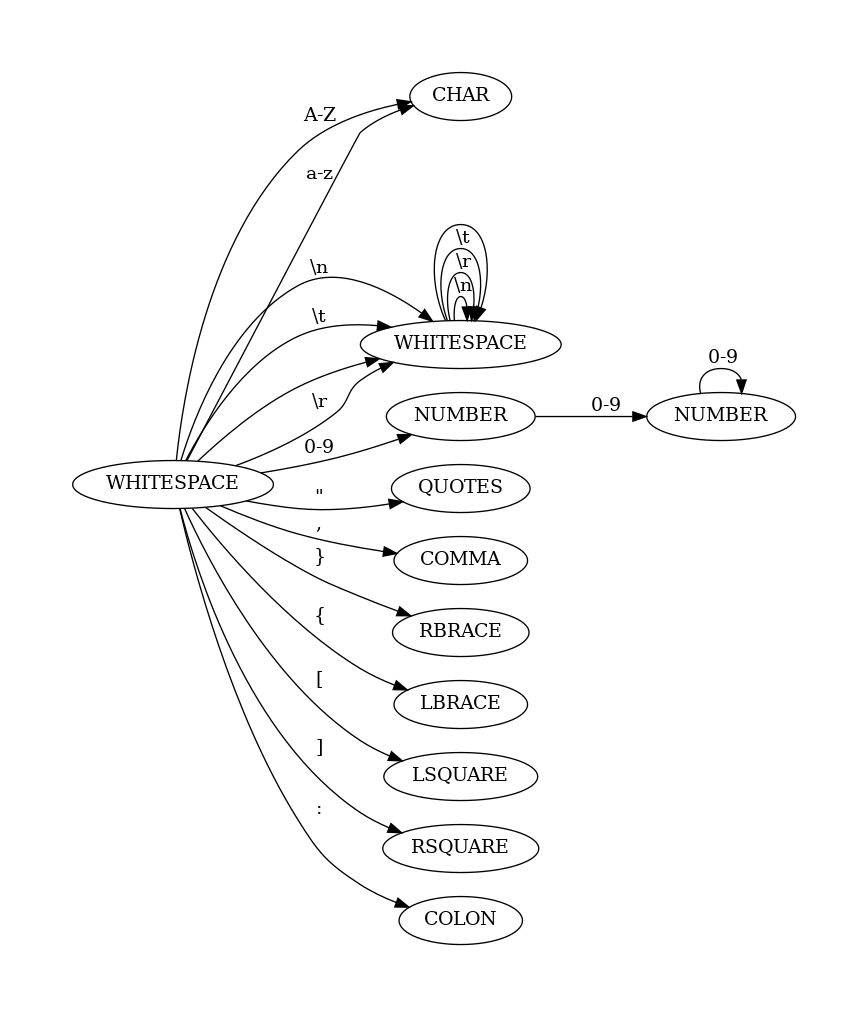
\includegraphics[width=\linewidth]{images/dfa.png}
\caption{DFA of the lexical grammar}
\label{fig:dfa}
\end{figure}

\begin{figure}[t]
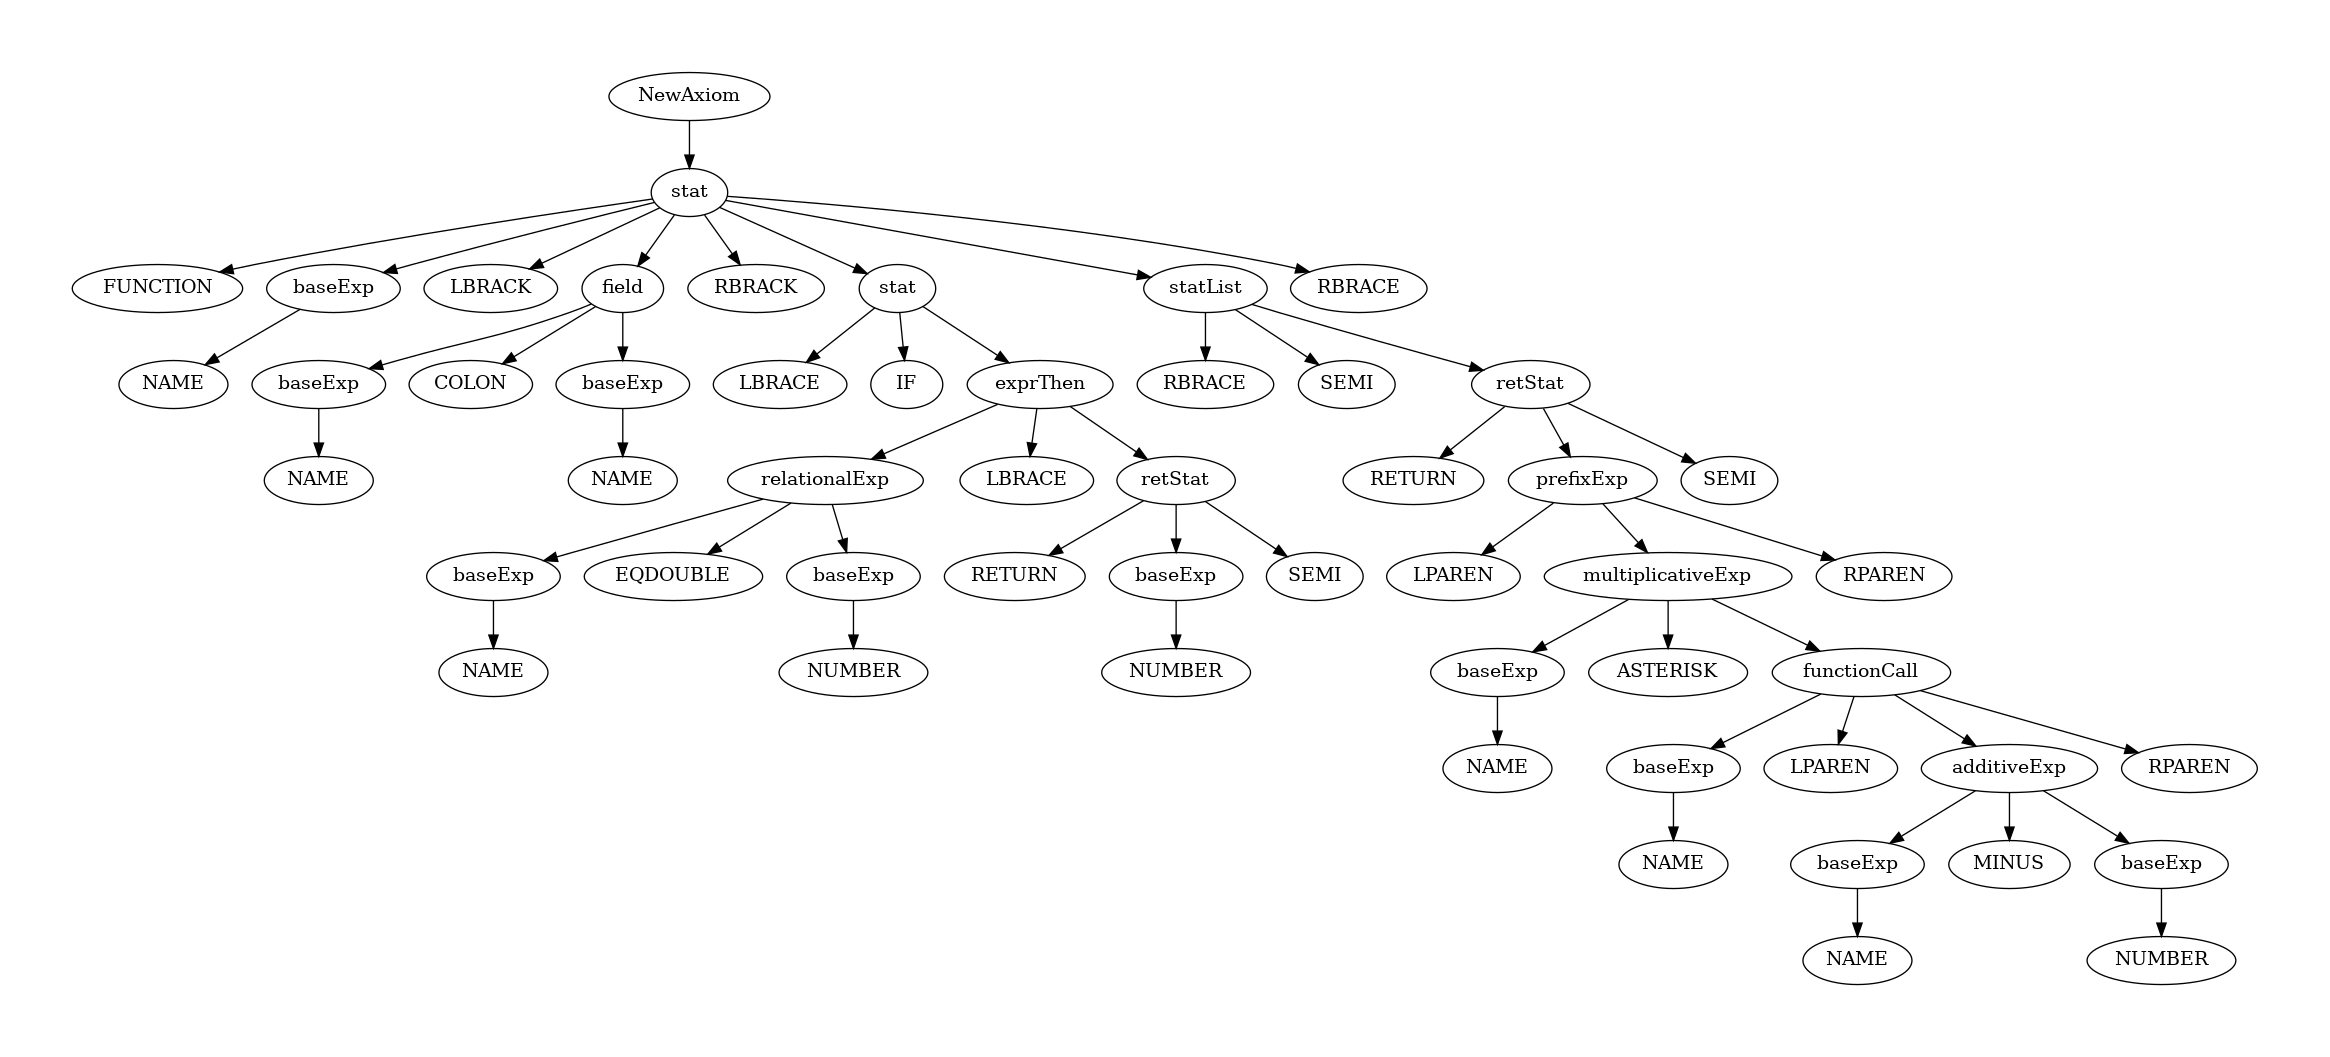
\includegraphics[width=\linewidth]{images/ptree.png}
\caption{Graphviz visualization of the parse tree.}
\label{fig:parse_tree}
\end{figure}

